% !Mode:: "TeX:UTF-8"
% !TEX program  = xelatex

\documentclass{report}

\title{复杂图像的直方图均衡、空域滤波与频域滤波设计与实现}
\stunum{第**组}
\stuname{{姓名1、姓名2、姓名3}}
\stuclass{计算机20**届**班}
\supervisor{*** \hspace{1.0em} 老师}
\dateinput{2026-04-15}

\begin{document}

\maketitle
\pagestyle{plain}
\pagenumbering{Roman}
\tableofcontents
\newpage
\pagestyle{plain}
\setcounter{page}{1}
\pagenumbering{arabic}

\section{团队成员分工}
\begin{itemize}
    \item 成员1：算法实现与实验。
    \item 成员2：结果整理与报告撰写。
    \item 成员3：测试与结果分析。
\end{itemize}

\section{任务背景}
数字图像在采集、传输和存储过程中往往会受到光照条件、传感器噪声以及成像系统分辨率的影响，导致图像出现对比度不足、噪声污染、边缘模糊等问题。为了提升图像的视觉质量，常常需要采用图像增强技术。图像增强方法大体可以分为空域方法和频域方法。空域方法直接对像素进行处理，具有直观、易实现的特点；频域方法则通过傅里叶变换将图像映射到频率空间，从频率分量角度实现平滑或锐化。

\section{任务描述}
本课程设计要求完成复杂图像的直方图均衡、空间滤波与频域滤波功能，具体包括：图像的直方图均衡；图像的线性平滑滤波与顺序统计滤波；图像的锐化滤波，包括拉普拉斯算子和一阶微分算子；基于傅里叶变换的频域低通滤波与高通滤波。同时，需要整理实现代码、实验结果和对比分析，形成完整报告。

\section{技术方案}
\subsection{方案总体架构}
本项目采用 Python 实现，使用 NumPy 完成矩阵与傅里叶运算，Pillow 负责图像读写，Matplotlib 用于绘制直方图和结果对比图。项目结构包括直方图处理模块、空域滤波模块、锐化模块、频域滤波模块以及实验脚本模块。实验脚本统一读取测试图像并自动输出处理结果，便于报告插图与分析。

\subsection{直方图均衡}
直方图均衡通过统计灰度分布并构造累积分布函数，将原始图像的灰度值重新映射到更均匀的分布上，从而提升整体对比度。设原始灰度级为 $r_k$，其概率分布为 $p(r_k)$，则变换函数可写为：
\[
s_k = T(r_k) = \sum_{j=0}^{k} p(r_j)
\]
实际实现中，再将累计概率线性映射到 $[0,255]$ 灰度范围。

\subsection{空间滤波}
线性平滑滤波采用均值模板对邻域像素求平均，用于抑制随机噪声，但会带来一定模糊。顺序统计滤波以邻域像素排序后的统计量替代中心像素，本实验实现了中值滤波。中值滤波对于椒盐噪声抑制效果明显，同时相比均值滤波更能保留边缘。

\subsection{锐化滤波}
图像锐化的目标是增强边缘和细节。本实验采用两类方法：一类是拉普拉斯二阶微分算子，通过增强灰度变化剧烈区域来突出边缘；另一类是一阶微分算子 Sobel，通过计算水平方向与垂直方向梯度来检测边缘，并将梯度响应叠加回原图完成增强。

\subsection{频域滤波}
频域滤波的核心是先对图像进行二维傅里叶变换，再在频谱平面中设计滤波器掩模。低通滤波保留低频成分，削弱高频噪声，因此可实现平滑；高通滤波则保留高频成分，突出边缘和纹理。实验中采用理想圆形低通和高通掩模进行演示。

\section{实验}
\subsection{数据集}
为了覆盖不同方法的特点，实验自建了 4 幅灰度测试图像：低对比度图像、椒盐噪声纹理图像、边缘块状图像以及周期纹理图像。低对比度图像用于展示直方图均衡效果，椒盐噪声图像用于比较均值滤波和中值滤波，边缘块状图像用于展示锐化效果，周期纹理图像用于分析频域滤波。

\subsection{评测指标}
本实验以定性分析为主，重点比较处理前后图像的视觉效果，包括对比度变化、噪声抑制能力、边缘增强程度以及不同频率成分被保留或削弱后的图像表现。同时辅以直方图和频谱图观察方法机理。

\subsection{实现细节}
项目包含 \texttt{histogram\_ops.py}、\texttt{spatial\_filters.py}、\texttt{sharpening.py} 和 \texttt{frequency\_filters.py} 四个核心模块，并编写 \texttt{run\_experiments.py} 对所有样例图像批量处理。为保证实现正确性，还使用 pytest 编写了 8 个基础测试，验证输出尺寸、数值范围以及中值滤波去除脉冲噪声等行为。

\subsection{定性实验}
\subsubsection{直方图均衡结果}
图~\ref{fig:hist} 给出了低对比度图像在直方图均衡前后的结果对比。可以看到，均衡后的图像层次更加分明，灰度分布范围明显扩展。

\begin{figure}[!h]
    \centering
    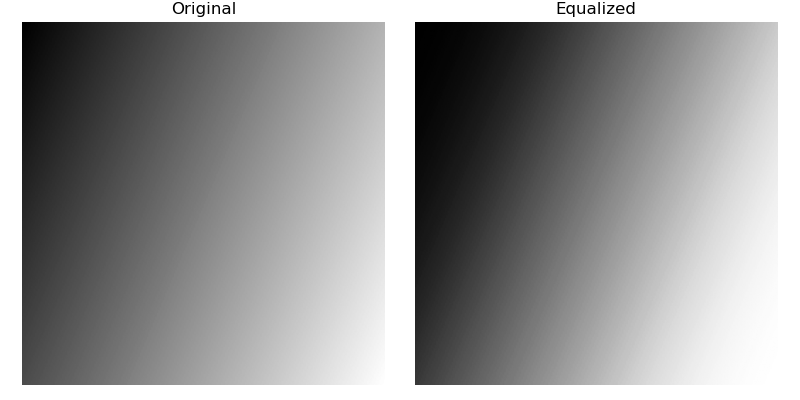
\includegraphics[width=0.85\textwidth]{figures/low_contrast_scene_histogram_compare}
    \caption{低对比度图像的直方图均衡结果对比}
    \label{fig:hist}
\end{figure}

\subsubsection{空间滤波结果}
图~\ref{fig:spatial} 展示了椒盐噪声图像经过均值滤波与中值滤波后的结果。均值滤波能够整体平滑图像，但会使边缘变钝；中值滤波对孤立噪声点的去除更明显，同时更好地保留了原始结构。

\begin{figure}[!h]
    \centering
    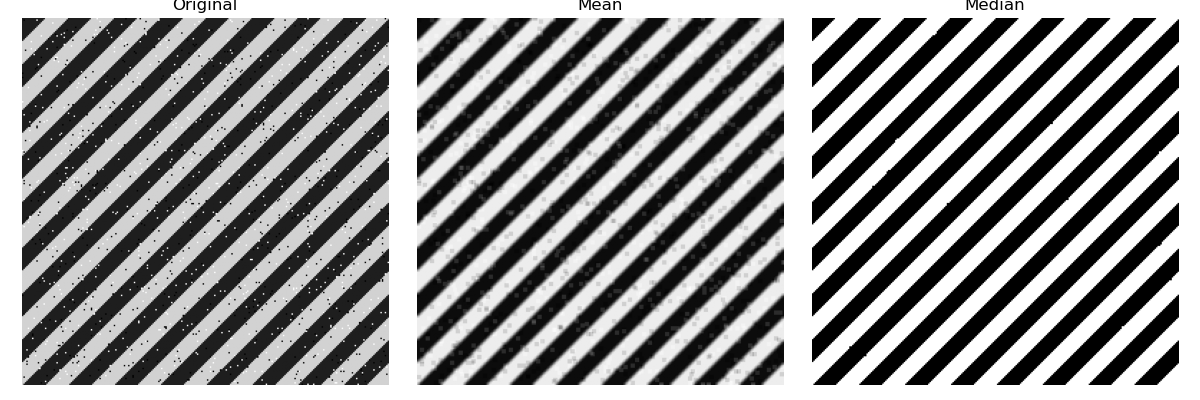
\includegraphics[width=0.85\textwidth]{figures/salt_pepper_texture_spatial_compare}
    \caption{椒盐噪声图像的空间滤波结果对比}
    \label{fig:spatial}
\end{figure}

\subsubsection{锐化滤波结果}
图~\ref{fig:sharp} 展示了边缘块状图像的锐化结果。拉普拉斯方法对灰度跃迁区域增强明显；Sobel 一阶微分则能够更稳定地提取方向性边缘信息，增强后的边界更加突出。

\begin{figure}[!h]
    \centering
    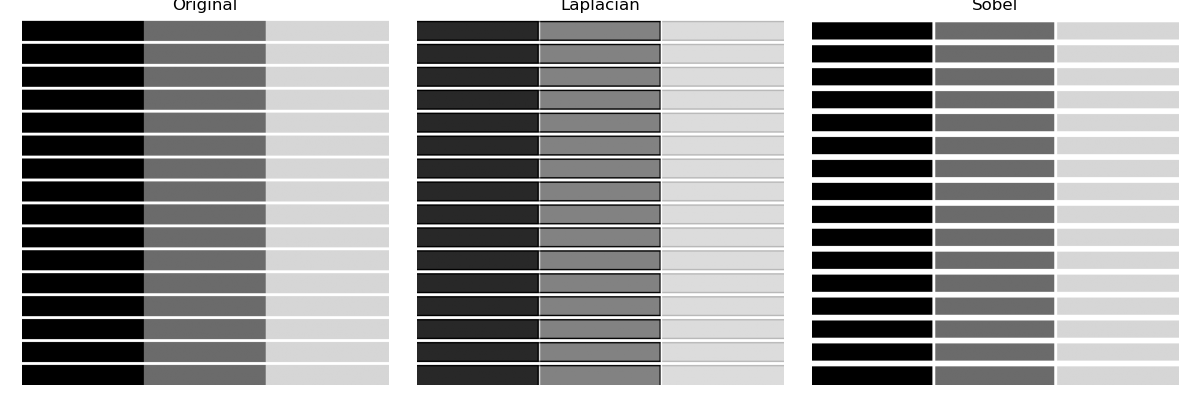
\includegraphics[width=0.85\textwidth]{figures/edge_blocks_sharpen_compare}
    \caption{边缘图像的锐化结果对比}
    \label{fig:sharp}
\end{figure}

\subsubsection{频域滤波结果}
图~\ref{fig:freq} 展示了周期纹理图像的低通与高通滤波结果。低通滤波保留整体亮度变化，削弱细密纹理；高通滤波则抑制低频背景，突出快速变化的条纹与边缘结构。

\begin{figure}[!h]
    \centering
    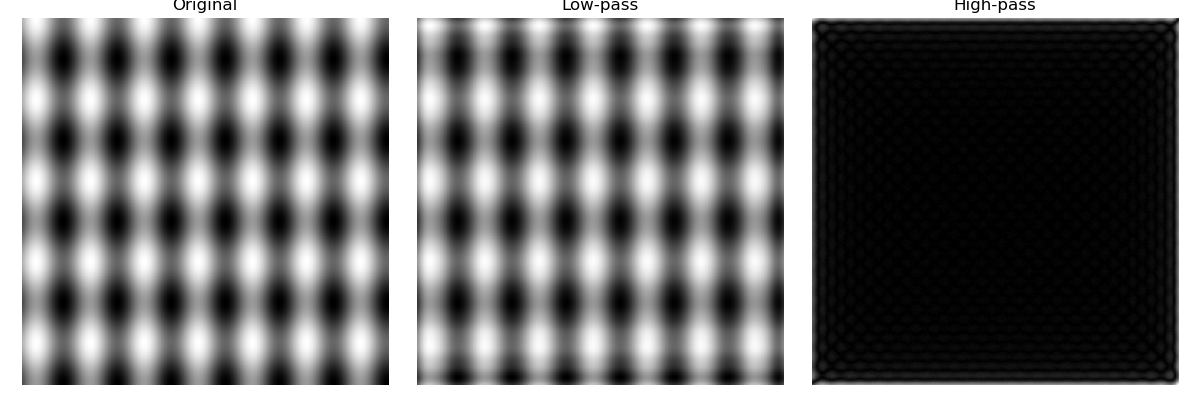
\includegraphics[width=0.85\textwidth]{figures/frequency_pattern_frequency_compare}
    \caption{周期纹理图像的频域滤波结果对比}
    \label{fig:freq}
\end{figure}

\subsection{结果分析比较}
综合实验结果可以看出，不同方法适用于不同任务。直方图均衡适合改善整体对比度不足的问题，但可能放大局部噪声；均值滤波适合削弱随机高频噪声，但会模糊边缘；中值滤波对于椒盐噪声表现更优；拉普拉斯和 Sobel 锐化都能增强边缘，但前者对噪声较敏感，后者具有更好的方向性；频域低通和高通则分别从频率角度实现平滑与增强，能够更直观体现图像不同频率成分的物理意义。

\section{总结}
本课程设计完成了直方图均衡、空域平滑滤波、顺序统计滤波、拉普拉斯锐化、一阶微分锐化以及基于傅里叶变换的低通和高通滤波等功能，并通过多组实验图像比较了各种方法的效果。实验表明，空域方法实现简单、便于理解，适合直接像素处理；频域方法更适合从整体频率分布角度分析图像。未来可以进一步扩展为彩色图像增强、自适应直方图均衡以及巴特沃斯、高斯频域滤波等更复杂的方法。

\end{document}
